\subsection*{Question 3.4}
The plot of the SVD.sampel, can be seen in figure \ref{fig:q34}, then the y axe is the diffrent geans, and the x axe is the distance betwin the diffrence grups. The longer out the geans is joint, the mor distance ther are betwin the geans. This representation, is are good wait to grup fing togget, sine we can set are max distian. and set are lien at thet distance, at jost finde alle the grupering that are to the left of the line. This also mean, that we can set are number of gruperings, and finde the distance the geans need to have to get the number og gruperings
\begin{figure}[!htbp]
  \centering
  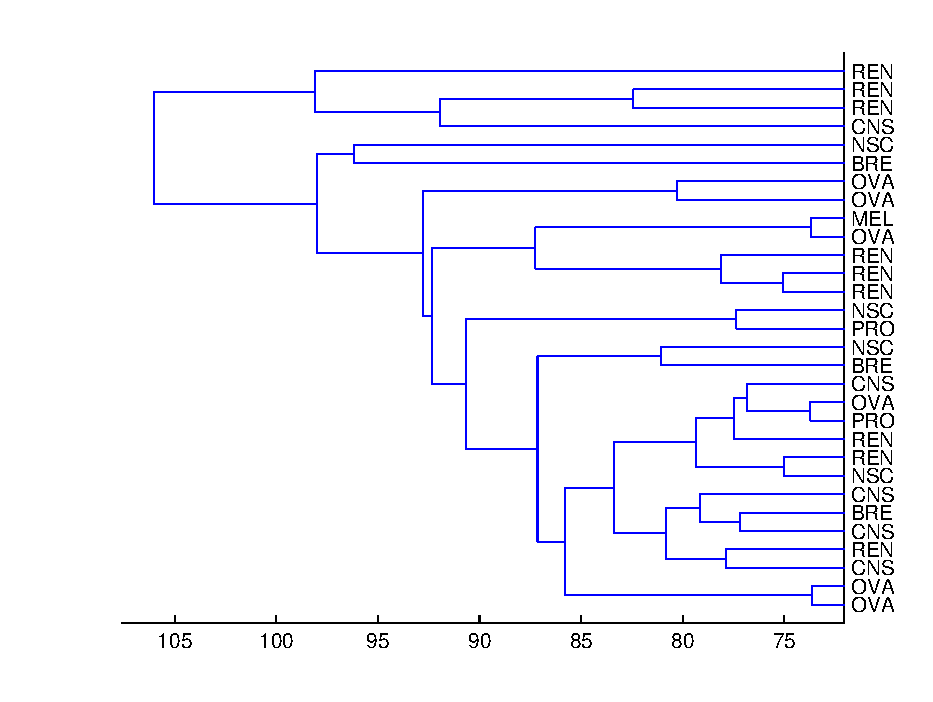
\includegraphics[width=0.85\textwidth]{./images/q34}
  \caption{Shows are plot over the first hand in the data set.}
  \label{fig:q34}
\end{figure}

